\documentclass[conference]{IEEEtran}
\usepackage{cite}
\usepackage{amsmath,amssymb,amsfonts}
\usepackage{graphicx}
\usepackage{booktabs}
\usepackage{tikz}
\usetikzlibrary{arrows.meta,positioning,shapes.geometric,fit}
\usepackage[hidelinks]{hyperref}

\def\BibTeX{{\rm B\kern-.05em{\sc i\kern-.025em b}\kern-.08em
    T\kern-.1667em\lower.7ex\hbox{E}\kern-.125emX}}

\begin{document}

\title{A Comparative Study of Deep Semantic Segmentation Architectures for
Geo-Referenced Road Extraction from Aerial Imagery}

\author{
\IEEEauthorblockN{Abhinav Shukla}
\IEEEauthorblockA{\textit{Department of Computer Science and Engineering}\\
\textit{Amity University}\\
Noida, India \\
abhinav@example.com}
\and
\IEEEauthorblockN{Faculty Guide Name}
\IEEEauthorblockA{\textit{Department of Computer Science and Engineering}\\
\textit{Amity University}\\
Noida, India \\
guide@example.com}
}

\maketitle

\begin{abstract}
Accurate and up-to-date road network information is essential for navigation,
urban planning, and disaster response, yet manual mapping cannot keep pace with
rapidly changing landscapes. This work presents a controlled comparative study
of four deep semantic segmentation architectures---U-Net, U-Net++, DeepLabV3+,
and LinkNet---for automated road extraction from high-resolution aerial
imagery. All models share an identical training protocol (encoder, loss,
optimizer, schedule, augmentation, and data), isolating the architecture as the
only experimental variable. On the Massachusetts Roads benchmark, U-Net++
achieves the best test accuracy (IoU $0.654$, $F_1$ $0.791$), while LinkNet
attains within $0.005$ IoU of the leader using the fewest parameters and the
fastest inference, revealing a practical accuracy--efficiency trade-off.
Beyond pixel accuracy, we integrate a geo-referencing pipeline that converts
detected road pixels into real-world coordinates using the imagery's embedded
geodetic metadata, exports vector GeoJSON, and validates the result against the
OpenStreetMap road network. The best model's geo-referenced output agrees with
OpenStreetMap as closely as the human-annotated ground truth does (correctness
$0.985$ vs.\ $0.979$), demonstrating that the extracted networks are directly
usable in geographic information systems.
\end{abstract}

\begin{IEEEkeywords}
road extraction, semantic segmentation, remote sensing, U-Net, deep learning,
geo-referencing, OpenStreetMap
\end{IEEEkeywords}

\section{Introduction}
The continuous growth of urban environments and transportation networks has
significantly increased the need for accurate, reliable, and frequently updated
road information. Road networks form the backbone of modern society, supporting
daily commuting, economic activity, emergency services, and large-scale
infrastructure planning. As cities expand and new routes are developed,
maintaining precise road data becomes both challenging and essential for
effective geographic management.

Satellite and aerial imagery provide comprehensive visual coverage across vast
geographic regions and have become a primary source of large-scale geographic
information for infrastructure monitoring and mapping
\cite{cheng2016survey,zhu2017deep}. Despite the availability of such rich data,
extracting meaningful information from imagery remains complex: traditional
manual digitization requires substantial human effort, consumes considerable
time, and cannot keep pace with rapidly changing landscapes.

Deep learning has opened new possibilities for automating the interpretation
of remote sensing data. Convolutional segmentation networks recognize intricate
spatial patterns, enabling fast and consistent identification of road
structures at scale \cite{long2015fcn,ronneberger2015unet}. However, published
road-extraction studies typically evaluate a single architecture under
author-specific training conditions, making reported accuracies difficult to
compare: differences may stem from the architecture, the loss function, the
augmentation policy, or simply the training budget. Moreover, most systems stop
at the pixel level---a binary mask in image space---leaving a gap between
detection and the geo-referenced vector data that mapping platforms and
geographic information systems (GIS) actually consume.

This work addresses both gaps with two contributions:
\begin{enumerate}
  \item \textbf{A controlled architecture comparison.} Four widely used
  segmentation architectures---U-Net \cite{ronneberger2015unet}, U-Net++
  \cite{zhou2018unetpp}, DeepLabV3+ \cite{chen2018deeplabv3plus}, and LinkNet
  \cite{chaurasia2017linknet}---are trained under a strictly identical
  protocol: the same ResNet-34 encoder, loss, optimizer, learning-rate
  schedule, augmentation, batch size, and data splits. Observed performance
  differences are therefore attributable to the decoder architecture alone.
  \item \textbf{An integrated geo-referencing pipeline.} Detected road masks
  are converted to real-world coordinates using the affine transform and
  coordinate reference system embedded in the source GeoTIFF imagery,
  vectorized to GeoJSON, rendered on interactive web maps, and quantitatively
  validated against the OpenStreetMap (OSM) road network.
\end{enumerate}

\section{Related Work}
Automated road extraction has been studied extensively in computer vision and
remote sensing \cite{mnih2010learning,mnih2013thesis,cheng2016survey}. An early
deep-learning breakthrough was DeepRoadMapper \cite{mattyus2017deeproadmapper},
which combined pixel-wise prediction from a convolutional network with graph
refinement to improve topological connectivity. RoadTracer
\cite{bastani2018roadtracer} instead constructed road graphs by iteratively
tracing paths across aerial imagery, emphasizing network formation over pixel
classification.

Fully convolutional networks \cite{long2015fcn} established dense prediction
as the dominant paradigm for segmentation. U-Net \cite{ronneberger2015unet},
originally designed for biomedical images, pairs a contracting encoder with a
symmetric decoder and skip connections that preserve fine spatial detail; its
data efficiency has made it a de facto standard for thin-structure
segmentation, including roads \cite{zhang2018resunet}. U-Net++
\cite{zhou2018unetpp} redesigns the skip pathways as nested, dense
convolutional blocks intended to reduce the semantic gap between encoder and
decoder features. DeepLabV3+ \cite{chen2017rethinking,chen2018deeplabv3plus}
employs atrous (dilated) convolution and spatial pyramid pooling to aggregate
multi-scale context without sacrificing resolution. LinkNet
\cite{chaurasia2017linknet} targets efficiency, linking each encoder stage
directly to its decoder counterpart to recover spatial information with few
parameters.

\textbf{Research gap.} These studies demonstrate strong detection accuracy,
but cross-paper comparisons are confounded by differing training conditions,
and limited attention has been paid to associating detections with precise
geographic coordinates. Outputs confined to the image domain are not directly
usable in mapping platforms. The present work contributes a like-for-like
architecture benchmark and closes the loop from pixels to geo-referenced,
OSM-validated vector data.

\section{Methodology}
Fig.~\ref{fig:pipeline} summarizes the proposed framework, from raw
georeferenced imagery to validated vector road networks.

\begin{figure}[t]
\centering
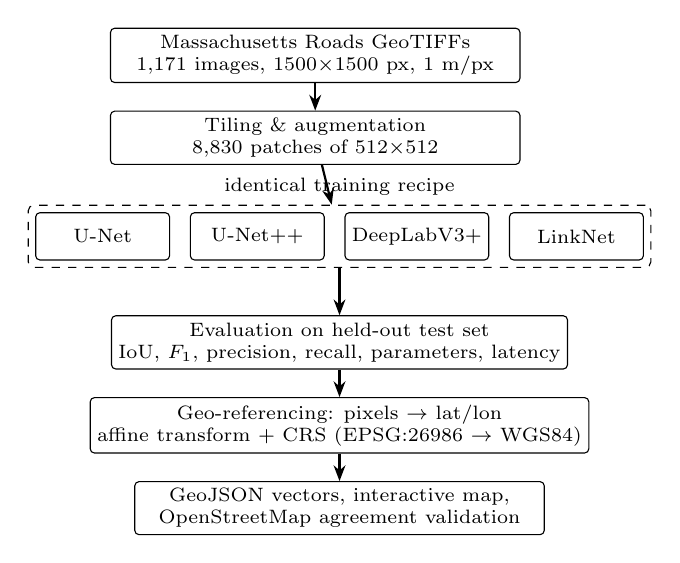
\begin{tikzpicture}[
  font=\scriptsize,
  node distance=3.5mm,
  box/.style={draw, rounded corners=1.5pt, align=center, inner sep=2.5pt,
              minimum height=6mm, minimum width=17mm},
  wide/.style={box, minimum width=52mm},
  arr/.style={-{Stealth[length=2mm]}, thick}
]
\node[wide] (data) {Massachusetts Roads GeoTIFFs\\ 1{,}171 images, $1500{\times}1500$ px, 1 m/px};
\node[wide, below=of data] (tile) {Tiling \& augmentation\\ $8{,}830$ patches of $512{\times}512$};
\node[box, below=6mm of tile, xshift=-27mm] (m1) {U-Net};
\node[box, right=2.5mm of m1] (m2) {U-Net++};
\node[box, right=2.5mm of m2] (m3) {DeepLabV3+};
\node[box, right=2.5mm of m3] (m4) {LinkNet};
\node[draw, dashed, rounded corners=2pt, inner sep=2.5pt,
      fit=(m1)(m2)(m3)(m4), label={[font=\scriptsize]above:{identical training recipe}}]
      (models) {};
\node[wide, below=6mm of models] (eval) {Evaluation on held-out test set\\ IoU, $F_1$, precision, recall, parameters, latency};
\node[wide, below=of eval] (geo) {Geo-referencing: pixels $\rightarrow$ lat/lon\\ affine transform + CRS (EPSG:26986 $\rightarrow$ WGS84)};
\node[wide, below=of geo] (out) {GeoJSON vectors, interactive map,\\ OpenStreetMap agreement validation};
\draw[arr] (data) -- (tile);
\draw[arr] (tile) -- (models);
\draw[arr] (models) -- (eval);
\draw[arr] (eval) -- (geo);
\draw[arr] (geo) -- (out);
\end{tikzpicture}
\caption{System overview. Four segmentation architectures are trained under an
identical protocol; the best model's predictions are geo-referenced and
validated against OpenStreetMap.}
\label{fig:pipeline}
\end{figure}

\subsection{Dataset and Preprocessing}
Experiments use the Massachusetts Roads Dataset \cite{mnih2013thesis},
comprising 1{,}171 aerial images of $1500\times1500$ pixels at 1\,m/pixel
resolution with pixel-level binary road annotations, split into 1{,}108
training, 14 validation, and 49 test images. The imagery is distributed as
GeoTIFF with an embedded affine transform in the NAD83 Massachusetts State
Plane coordinate system (EPSG:26986), which our geo-referencing stage exploits
directly.

Each image is cut into a $3\times3$ grid of $512\times512$ patches with slight
overlap. Patches in which more than 25\% of pixels are blank (white no-data
padding present at collection boundaries) are discarded, yielding 8{,}263
training, 126 validation, and 441 test tiles. Training-time augmentation
comprises horizontal/vertical flips, $90^{\circ}$ rotations, and random
brightness--contrast jitter; images are normalized with ImageNet statistics.

\subsection{Architectures Compared}
All four models are encoder--decoder segmentation networks instantiated with
the same ImageNet-pretrained ResNet-34 encoder \cite{he2016resnet}, differing
only in decoder design: U-Net's symmetric decoder with plain skip connections
\cite{ronneberger2015unet}; U-Net++'s nested, densely connected skip pathways
\cite{zhou2018unetpp}; DeepLabV3+'s atrous spatial pyramid pooling
\cite{chen2018deeplabv3plus}; and LinkNet's lightweight additive decoder
\cite{chaurasia2017linknet}.

\subsection{Identical Training Protocol}
Every model is trained with the combined Dice and binary cross-entropy
objective
\begin{equation}
\mathcal{L} = \tfrac{1}{2}\,\mathcal{L}_{\mathrm{Dice}} +
              \tfrac{1}{2}\,\mathcal{L}_{\mathrm{BCE}},
\end{equation}
which is well suited to thin structures occupying a small fraction of pixels
(roads cover ${\sim}5\%$ of the dataset). Optimization uses AdamW (learning
rate $3\times10^{-4}$, weight decay $10^{-4}$) with cosine annealing over 30
epochs at batch size 8 and a fixed random seed. The checkpoint with the best
validation IoU is retained. Training was performed on freely available NVIDIA
T4 GPUs (Kaggle), each model completing in 2.5--9 hours.

\subsection{Evaluation Metrics}
Let TP, FP, and FN denote pixel-level true positives, false positives, and
false negatives aggregated over the test set. We report intersection over
union $\mathrm{IoU} = \mathrm{TP}/(\mathrm{TP}+\mathrm{FP}+\mathrm{FN})$,
$F_1$ (Dice), precision, and recall, together with parameter counts and
per-tile inference latency.

\subsection{Geo-Referencing and OSM Validation}
The predicted binary mask of a full image is vectorized into polygons, whose
vertices are mapped from pixel space to projected coordinates by the GeoTIFF
affine transform and then to WGS84 longitude/latitude. The result is exported
as GeoJSON and rendered over OpenStreetMap tiles for interactive inspection.

For quantitative validation, all OSM ways tagged \texttt{highway} within the
image footprint are retrieved via the Overpass API, projected to the image
grid, and buffered by 6\,m. We then compute \emph{correctness}, the fraction
of predicted road pixels lying within the buffered OSM network (does the model
invent roads?), and \emph{completeness}, the fraction of the buffered OSM
network covered by the prediction (how much of the mapped network is
recovered?). Because OSM's \texttt{highway} tag includes footpaths and service
ways that are frequently invisible in 1\,m aerial imagery, we additionally
report the same measures for the human-annotated ground truth as an achievable
upper reference.

\section{Results and Discussion}

\subsection{Segmentation Accuracy}
Table~\ref{tab:comparison} reports test-set performance. All four
architectures land in a narrow, competitive band (IoU
$0.642$--$0.654$), consistent with published results on this benchmark and
confirming that, under equal training conditions, decoder design produces
measurable but moderate differences.

\begin{table}[t]
\caption{Test-Set Comparison on the Massachusetts Roads Dataset
(441 tiles; identical training protocol). Latency measured per
$512\times512$ tile on an Apple-silicon MPS device.}
\label{tab:comparison}
\centering
\footnotesize
\setlength{\tabcolsep}{3.5pt}
\begin{tabular}{@{}lcccccc@{}}
\toprule
Model & IoU & $F_1$ & Prec. & Rec. & Par.\ (M) & ms \\
\midrule
U-Net++      & \textbf{0.654} & \textbf{0.791} & \textbf{0.808} & \textbf{0.774} & 26.1 & 199.8 \\
U-Net        & 0.650 & 0.788 & 0.807 & 0.770 & 24.4 & 110.5 \\
LinkNet      & 0.649 & 0.787 & 0.803 & 0.771 & \textbf{21.8} & \textbf{105.0} \\
DeepLabV3+   & 0.642 & 0.782 & 0.798 & 0.766 & 22.4 & 117.5 \\
\bottomrule
\end{tabular}
\end{table}

U-Net++ attains the best accuracy on every metric, supporting the hypothesis
that its nested skip pathways reduce the encoder--decoder semantic gap and
benefit thin-structure localization---but at nearly double the inference
latency of the alternatives. LinkNet is the clear efficiency choice: within
$0.005$ IoU of the leader while using 16\% fewer parameters and running
$1.9\times$ faster than U-Net++. DeepLabV3+, whose atrous pyramid excels on
large-object benchmarks, trails here; aggressive context aggregation appears
less advantageous for one-meter-wide linear structures than high-resolution
skip connections. Precision exceeds recall for all models, indicating
conservative predictors whose residual errors are dominated by missed narrow
or occluded roads rather than hallucinated ones.

\begin{figure}[t]
\centering
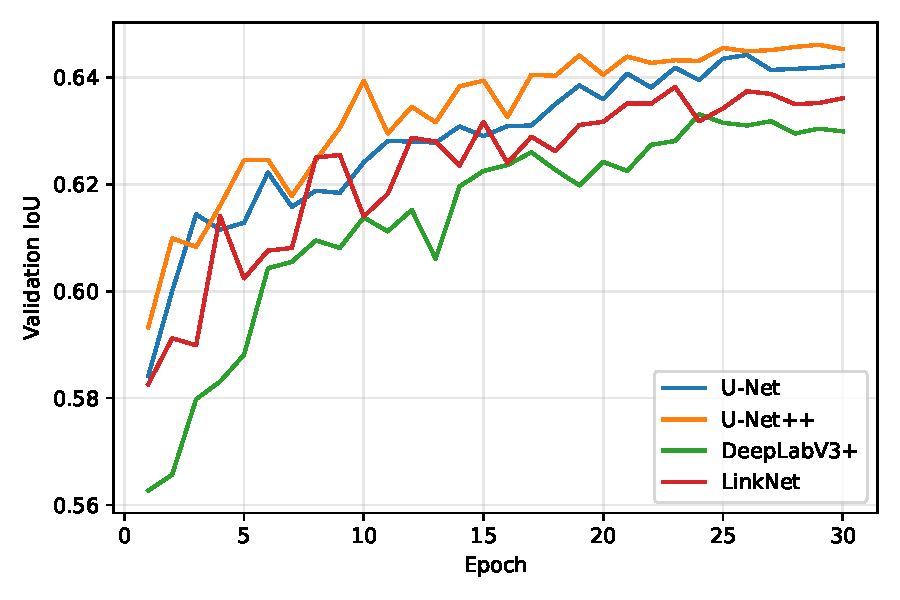
\includegraphics[width=\columnwidth]{figures/val_iou_curves.pdf}
\caption{Validation IoU per epoch under the identical training protocol. All
models converge stably; U-Net++ overtakes U-Net in the final third of
training.}
\label{fig:curves}
\end{figure}

Fig.~\ref{fig:curves} shows validation IoU over training. Convergence is
smooth for all models; U-Net leads early, but U-Net++ continues improving and
overtakes it after epoch ${\sim}25$, suggesting the denser decoder benefits
from a longer optimization horizon.

\begin{figure*}[t]
\centering
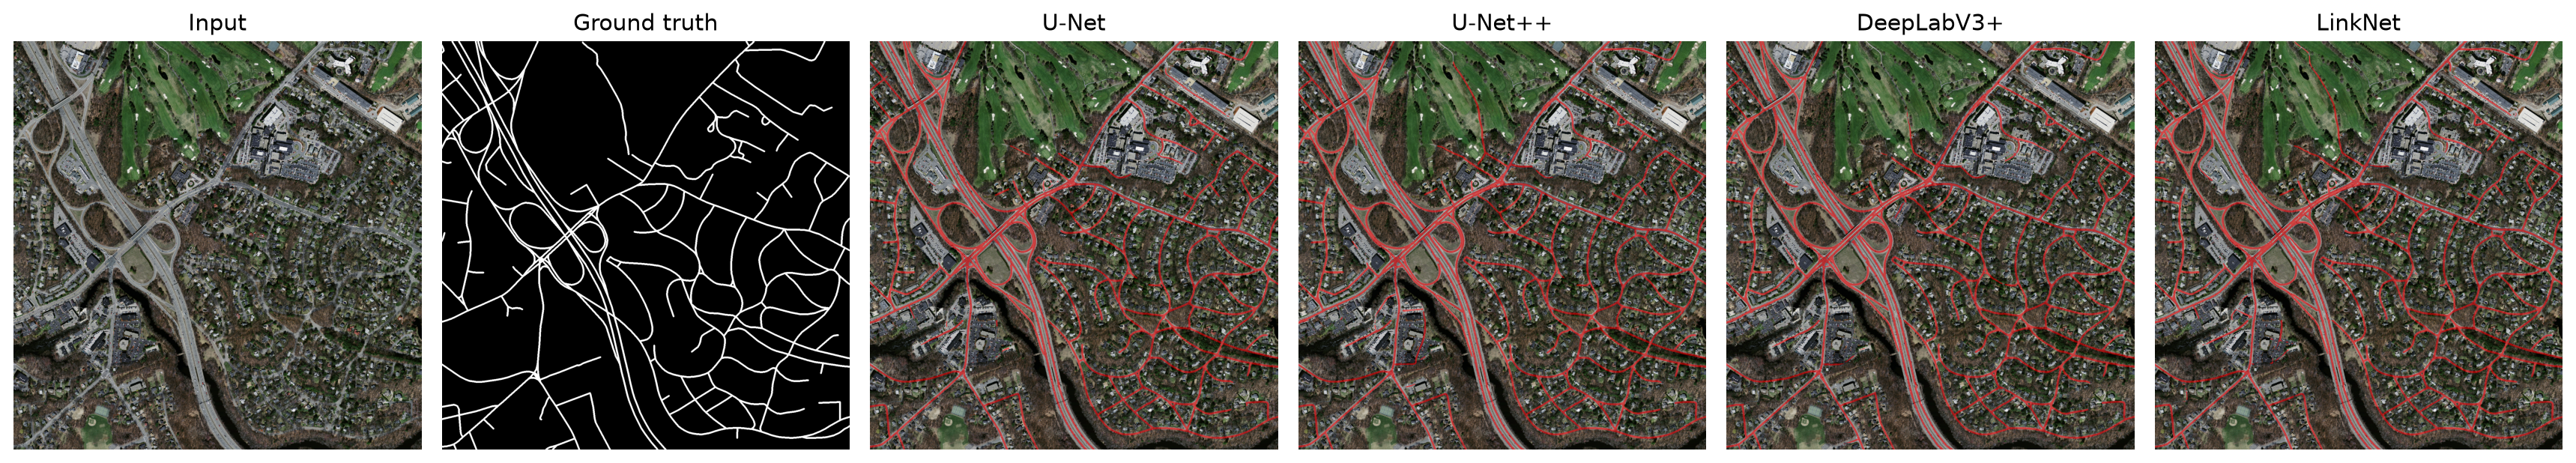
\includegraphics[width=\textwidth]{figures/qualitative_22078975_15.png}
\caption{Qualitative comparison on a full $1500\times1500$ test image
(suburban Newton, MA, including a highway interchange). Left to right: input
image, human ground truth, and predictions (red overlay) of the four models.
All architectures recover the arterial network; differences concentrate in
narrow residential streets and partially occluded segments.}
\label{fig:qualitative}
\end{figure*}

Fig.~\ref{fig:qualitative} presents a qualitative comparison. All models
recover the interchange and arterial roads; disagreements concentrate in
tree-occluded residential streets---the same regions where the models'
recall deficit originates.

\subsection{Geo-Referenced Output and OSM Agreement}
Applying the geo-referencing stage to the U-Net++ prediction of the
Fig.~\ref{fig:qualitative} scene ($42.321^{\circ}$--$42.335^{\circ}$\,N,
$71.239^{\circ}$--$71.258^{\circ}$\,W) yields 28 road polygons in GeoJSON,
rendered interactively over OpenStreetMap. Table~\ref{tab:osm} summarizes the
agreement between the geo-referenced prediction and 916 OSM ways retrieved for
the scene.

\begin{table}[t]
\caption{Agreement with the OpenStreetMap Road Network (6 m buffer).}
\label{tab:osm}
\centering
\begin{tabular}{@{}lcc@{}}
\toprule
Source & Correctness & Completeness \\
\midrule
U-Net++ prediction        & \textbf{0.985} & \textbf{0.320} \\
Human ground truth        & 0.979 & 0.316 \\
\bottomrule
\end{tabular}
\end{table}

Two observations follow. First, correctness of $0.985$ means virtually every
pixel the model labels as road lies within 6\,m of a mapped OSM road: the
geo-referencing chain (prediction $\rightarrow$ affine transform
$\rightarrow$ datum conversion) is spatially accurate, and the model does not
hallucinate geometry. Second, the prediction's completeness ($0.320$)
\emph{matches the human ground truth's} ($0.316$): the apparently low value is
explained by OSM footpaths, driveways, and service ways that are absent from
both the imagery-derived annotation and the prediction, not by model failure.
By this measure, the automatically extracted, geo-referenced network is as
consistent with OSM as the manual annotation it was trained on.

\section{Conclusion}
This paper presented a controlled comparison of four semantic segmentation
architectures for road extraction, trained under a strictly identical
protocol on the Massachusetts Roads Dataset, together with a geo-referencing
pipeline that converts predictions into GIS-ready, OSM-validated vector data.
U-Net++ achieved the best accuracy (test IoU $0.654$), while LinkNet offered
near-identical accuracy at the lowest computational cost, a relevant result
for large-area or on-board processing. The geo-referenced output of the best
model agreed with OpenStreetMap as closely as the human ground truth,
demonstrating end-to-end fidelity from pixels to coordinates.

Future work includes topology-aware losses and relaxed (buffer-based)
evaluation to better reflect connectivity, transformer-based encoders,
skeletonization to centerline vectors for direct map conflation, and scaling
the pipeline to national road inventories using satellite constellations.

\begin{thebibliography}{00}
\bibitem{ronneberger2015unet} O. Ronneberger, P. Fischer, and T. Brox,
``U-Net: Convolutional networks for biomedical image segmentation,'' in
\emph{Proc. MICCAI}, 2015, pp. 234--241.
\bibitem{zhou2018unetpp} Z. Zhou, M. M. Rahman Siddiquee, N. Tajbakhsh, and
J. Liang, ``UNet++: A nested U-Net architecture for medical image
segmentation,'' in \emph{Proc. DLMIA/MICCAI Workshops}, 2018, pp. 3--11.
\bibitem{chen2018deeplabv3plus} L.-C. Chen, Y. Zhu, G. Papandreou, F. Schroff,
and H. Adam, ``Encoder--decoder with atrous separable convolution for semantic
image segmentation,'' in \emph{Proc. ECCV}, 2018, pp. 801--818.
\bibitem{chaurasia2017linknet} A. Chaurasia and E. Culurciello, ``LinkNet:
Exploiting encoder representations for efficient semantic segmentation,'' in
\emph{Proc. IEEE VCIP}, 2017, pp. 1--4.
\bibitem{chen2017rethinking} L.-C. Chen, G. Papandreou, F. Schroff, and
H. Adam, ``Rethinking atrous convolution for semantic image segmentation,''
\emph{arXiv:1706.05587}, 2017.
\bibitem{mattyus2017deeproadmapper} G. M\'attyus, W. Luo, and R. Urtasun,
``DeepRoadMapper: Extracting road topology from aerial images,'' in
\emph{Proc. IEEE ICCV}, 2017, pp. 3438--3446.
\bibitem{bastani2018roadtracer} F. Bastani \emph{et al.}, ``RoadTracer:
Automatic extraction of road networks from aerial images,'' in \emph{Proc.
IEEE CVPR}, 2018, pp. 4720--4728.
\bibitem{mnih2010learning} V. Mnih and G. E. Hinton, ``Learning to detect
roads in high-resolution aerial images,'' in \emph{Proc. ECCV}, 2010,
pp. 210--223.
\bibitem{mnih2013thesis} V. Mnih, ``Machine learning for aerial image
labeling,'' Ph.D. dissertation, Univ. of Toronto, 2013.
\bibitem{long2015fcn} J. Long, E. Shelhamer, and T. Darrell, ``Fully
convolutional networks for semantic segmentation,'' in \emph{Proc. IEEE CVPR},
2015, pp. 3431--3440.
\bibitem{he2016resnet} K. He, X. Zhang, S. Ren, and J. Sun, ``Deep residual
learning for image recognition,'' in \emph{Proc. IEEE CVPR}, 2016,
pp. 770--778.
\bibitem{zhang2018resunet} Z. Zhang, Q. Liu, and Y. Wang, ``Road extraction by
deep residual U-Net,'' \emph{IEEE Geosci. Remote Sens. Lett.}, vol. 15, no. 5,
pp. 749--753, 2018.
\bibitem{cheng2016survey} G. Cheng and J. Han, ``A survey on object detection
in optical remote sensing images,'' \emph{ISPRS J. Photogramm. Remote Sens.},
vol. 117, pp. 11--28, 2016.
\bibitem{zhu2017deep} X. X. Zhu \emph{et al.}, ``Deep learning in remote
sensing: A comprehensive review and list of resources,'' \emph{IEEE Geosci.
Remote Sens. Mag.}, vol. 5, no. 4, pp. 8--36, 2017.
\end{thebibliography}

\end{document}
